\documentclass[a4paper, 12pt]{article}%тип документа

%%%Библиотеки
	%\usepackage[warn]{mathtext}	
	\usepackage[T2A]{fontenc} % кодировка
	\usepackage[utf8]{inputenc} % кодировка исходного текста
	\usepackage[english,russian]{babel} % локализация и переносы
	\usepackage{caption}
	\usepackage{listings}
	\usepackage{amsmath,amsfonts,amssymb,amsthm,mathtools}
	\usepackage{wasysym}
	\usepackage{graphicx}%Вставка картинок правильная
	\usepackage{float}%"Плавающие" картинки
	\usepackage{wrapfig}%Обтекание фигур (таблиц, картинок и прочего)
	\usepackage{fancyhdr} %загрузим пакет
	\usepackage{lscape}
	\usepackage{xcolor}
	\usepackage[normalem]{ulem}
	\usepackage{hyperref}

%%%Конец библиотек




%%%Настройка ссылок
	\hypersetup
	{
		colorlinks=true,
		linkcolor=blue,
		filecolor=magenta,
		urlcolor=blue
	}
%%%Конец настройки ссылок


%%%Настройка колонтитулы
	\pagestyle{fancy}
	\fancyhead{}
	\fancyhead[L]{Лабораторная работа}
	\fancyhead[R]{Талашкевич Даниил, группа Б01-009}
	\fancyfoot[C]{\thepage}
%%%конец настройки колонтитулы



							\begin{document}
						%%%%Начало документа%%%%


%%%Начало титульника
\begin{titlepage}

	\newpage
	\begin{center}
		\normalsize Московский физико-технический институт \\(госудраственный 			университет)
	\end{center}

	\vspace{6em}

	\begin{center}
		\Large Лабораторная работа по электричеству\\
	\end{center}

	\vspace{1em}

	\begin{center}
		\large \textbf{Релаксационные колебания [3.2.8]}
	\end{center}

	\vspace{2em}

	\begin{center}
		\large Талашкевич Даниил Александрович\\
		Группа Б01-009
	\end{center}

	\vspace{\fill}

	\begin{center}
	Долгопрудный \\2021
	\end{center}
	
\end{titlepage}
%%%Конец Титульника



%%%Настройка оглавления и нумерации страниц
	\thispagestyle{empty}
	\newpage
	\tableofcontents
	\newpage
	\setcounter{page}{1}
%%%Настройка оглавления и нумерации страниц


					%%%%%%Начало работы с текстом%%%%%%

\section{Аннотация}

В работе предлагается снять вольт-амперную характеристику стабилитрона и познакомиться с работой релаксационного генератора: определить критическое сопротивление, исследовать зависимость периода колебаний от сопротивления при фиксированной ёмкости и от ёмкости при фиксированном сопротивлении.

\section{Теоретические сведения}

 Колебательные системы, как правило, имеют два накопителя, между которыми происходит перекачка энергии. В контуре, содержащем конденсатор и катушку индуктивности, электрическая энергия переходит в магнитную и обратно; при колебаниях маятника потенциальная энергия поля тяжести переходит в кинетическую энергию движущейся массы и т.д. 

\begin{wrapfigure}{r}{0.3\textwidth} 
\begin{center}
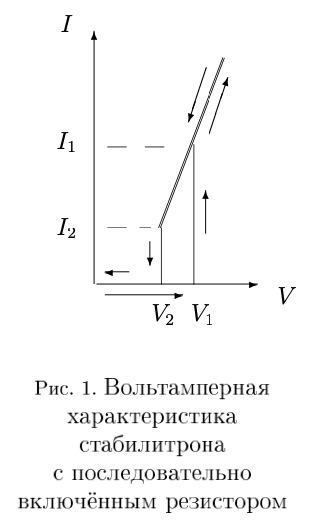
\includegraphics[width=0.3\textwidth]{./ann/1.PNG} 
\end{center}
\end{wrapfigure}

Встречаются, однако, колебательные системы, содержащие всего один накопитель энергии. Рассмотрим в качестве примера электрическую цепь, содержащую конденсатор и сопротивление без самоиндукции. Разряд конденсатора через сопротивление представляет собой апериодический процесс. Разряду, однако, можно придать периодический характер, возобновляя заряд конденсатора через постоянные промежутки времени. Колебания в этом случае являются совокупностью двух апериодических процессов - процесса зарядки конденсатора и процесса его разрядки. Такие колебания называются релаксационними.\\
В нашей установке роль ключа, обеспечивающего последовательно попеременную зарядку и разрядку конденсатора, играет газоразрядный диод. Зависимость тока от напряжения для газоразрядной лампы не подчиняется закону Ома и характеризуется рядом особенностей (рис. 1). При малых напряжениях лампа не пропускает тока вовсе (не горит). Ток в лампе возникает только в том случае, если разность потенциалов на её электродах достигает напряжения зажигания $V_{1} .$ При этом, тлеюиций разряд. При дальнейшем незначительном увеличении напряжения сила тока заметно возрастает по закону, близкому к линейному. 
Если начать уменьшать напряжение на горящей лампе, то при напряжении, равном $V_{1},$ лампа ещё не гаснет, и сила тока продолжает уменьшаться. Лампа перестанет пропускать ток лишь при напряжении гашения $V_{2},$ которое обычно существенно меньше $V_{1}$. Сила тока при этом скачком падает от значения $I_{2}\left(I_{2}<I_{1}\right)$ до нуля. Характеристика, изображённая на рис. 1, несколько идеализирована. $\mathrm{Y}$ реальной лампы зависимость $I(V)$ не вполне линейна. При $V>V_{1}$ графики
соответствующие возрастанию и убыванию напряжения, не всегда совпадают. Эти отличия, впрочем, носят второстепенный характер и для нашей задачи несущественны.
 
\newpage

\begin{wrapfigure}{r}{0.3\textwidth} 
\begin{center}
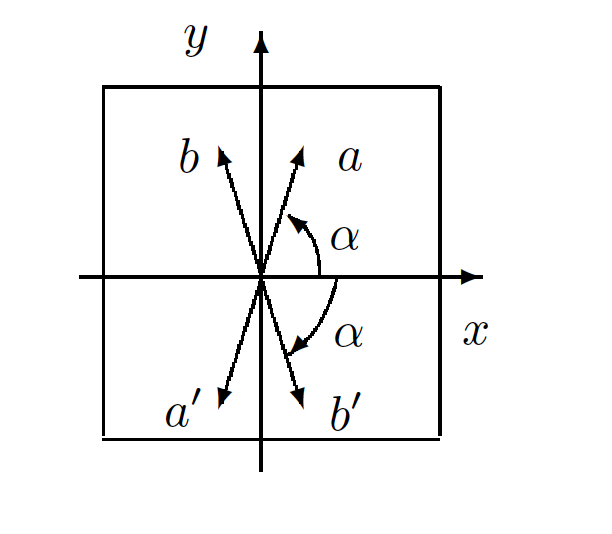
\includegraphics[width=0.3\textwidth]{./ann/2.PNG} 
\end{center}
\end{wrapfigure}


Рассмотрим схему релаксационного генератора, представленную на рис. $2 .$ Пусть напряжение бата- реи $U$ больше напряжения зажигания $V_{1} .$ В обозначениях, принятых на схеме, справедливо уравнение

$$I_{C}+I(V)=\frac{U-V}{R}$$

$$C \frac{d V}{d T}+I(V)=\frac{U-V}{R}$$
\\

В стационарном режиме работы, когда напряжение $V$ на конденсаторе постоянно и $d V / d t=0,$ ток через лампу равен

$$I_{\mathrm{cr}}=\frac{U-V}{R}$$

\begin{wrapfigure}{r}{0.3\textwidth} 
\begin{center}
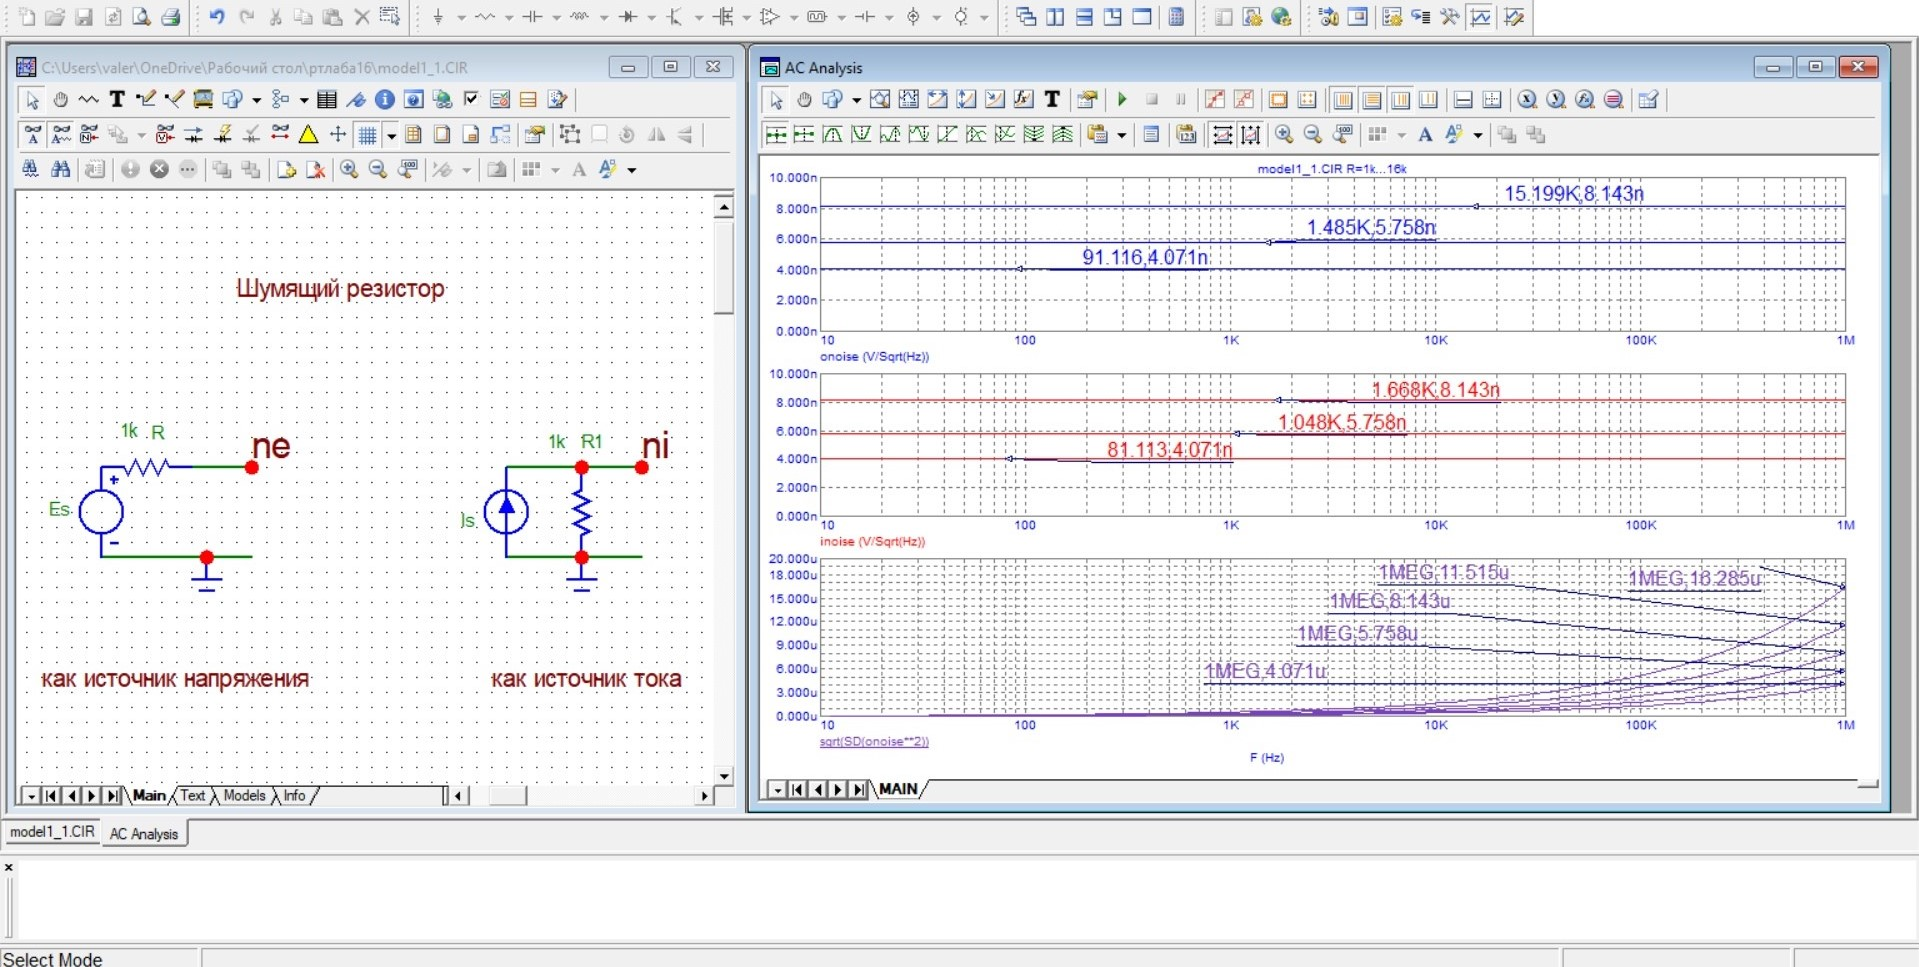
\includegraphics[width=0.3\textwidth]{./ann/3.PNG} 
\end{center}
\end{wrapfigure}

Равенство (2) может быть представлено графически (рис. 3) При разных $R$ графрики имеют вид прямых, пересекаЮщихся в точке $V=U, I=0 .$ Область, где эти иагрузочиъе прямвие пересекают вольт-амперную характеристику лампы, соответствует стационарному режиму - при малых $R$ (прямая 1$)$ лампа горит постоянно, колебания Отсутствуют. Прямая $2,$ проходящая через точку $\left(I_{2}, V_{2}\right),$ соответствует критическому сопротивлению
$$
R_{\mathrm{Kp}}=\frac{U-V_{2}}{I_{2}}
$$
При сопротивлении $R>R_{\text {кр }}$ нагрузочная прямая $3 \quad$ не пересекает характеристику лампы, поэтому стационарный режим невозможен. В этом случае в системе устанавливаются колебания. Рассмотрим, как происходит колебательный процесс. Пусть в начале опыта ключ К разомкнут (рис. 2) и $V=0 .$ Замкнём ключ. Конденсатор $C$ начинает заряжаться через сопротивление $R,$ напряжение на нём увеличивается (рис. 4) Как только оно достигнет напряжения зажигания $V_{1},$ лампа начинает проводить ток, причём прохождение тока сопровождается разрядкой конденсатора. В самом деле, батарея $U,$ подключённая через большое сопротивление $R,$ не может поддерживать необходимую для горения лампы величину тока. Во время горения лампы конденсатор разряжается, и когда напряжение на нём достигнет потенциала гашения, лампа перестанет проводить ток, а конденсатор вновь начнёт заряжаться. Возникают релаксационные колебания с амплитудой, равной $\left(V_{1}-V_{2}\right) .$

\newpage

\begin{wrapfigure}{r}{0.3\textwidth} 
\begin{center}
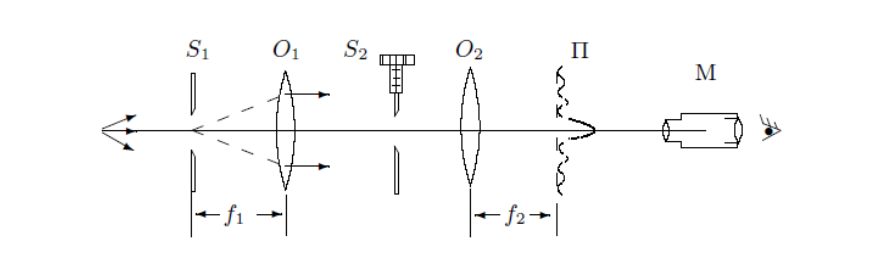
\includegraphics[width=0.3\textwidth]{./ann/4.PNG} 
\end{center}
\end{wrapfigure}

Рассчитаем период колебаний. Полное время одного периода колебаний Т состоит из суммы времени зарядки $\tau_{3}$ и времени разрядки $\tau_{\mathrm{p}},$ но если сопротивление $R$ существенно превосходит сопротивление Зажжённой лампы, то $\tau_{3} \gg \tau_{\mathrm{p}}$ и $T \simeq \tau_{3}($ этим случаем мы и ограничимся). Во время зарядки конденсатора лампа не горит $[I(V)=0],$ и уравнение (1) приобретает вид
$$
R C \frac{d V}{d t}=U-V
$$
Будем отсчитывать время с момента гашения лампы, так что $V=V_{2}$ при $t=0$ (рис. 4$) .$ Решив уравнение $(4),$ найдём
$$
V=U-\left(U-V_{2}\right) e^{-t /(R C)}
$$
$\mathrm{B}$ момент зажигания $t=\tau_{3}, V=V_{1},$ поэтому
$$
V_{1}=U-\left(U-V_{2}\right) e^{-\tau_{3} /(R C)}
$$
Из уравнений (5) и (6) нетрудно найти период колебаний:
$$
T \approx \tau_{3}=R C \ln \frac{U-V_{2}}{U-V_{1}}
$$
Развитая выше теория является приближённой. Ряд принятых при расчётах упрощающих предположений оговорен в тексте. Следует иметь в виду, что мы полностью пренебрегли паразитными емкостями и индуктивностями схемы. Не
рассматривались также процессы развития разряда и деионизация при гашении. Поэтому теория справедлива лишь в тех случаях, когда в схеме установлена достаточно большая ёмкость и когда период колебаний существенно больше времени развития разряда и времени деионизации (практически $\gg 10^{-5}$ с). Кроме того, потенциал гашения $V_{2},$ взятый из статической вольт-амперной характеристики, может отличаться от потенциала гашения лампы, работающей в динамическом режиме релаксационных колебаний.

\section{Результаты измерений и обработка данных}

YUYYY

\section{Обработка результатов}


$$\frac{\Delta V_{д}}{V_{д}} = \sqrt{\left(\frac{\Delta U}{U} \right)^2 + \left(\frac{\Delta V_1}{V_1} \right)^2 + \left(\frac{\Delta R}{R} \right)^2 + \left(\frac{\Delta C}{C} \right)^2 + \left(\frac{\Delta T}{T} \right)^2} \approx  \frac{\Delta T}{T}  \approx xx\%$$

\section{Вывод}

Мы познакомились с работой релаксационного генератора и определили все характеризующие его параметры.  Выяснилось, что теоретические рассчеты немногим отличаются от действительности, например Динамический потенциал гашения отличается на 7\%. 


\section{Литература}

\begin{enumerate}
\item \textbf{Лабораторный практикум по общей физике:} учеб. пособие. В трёх томах. Т. 2. Электричество и магнетизм /
Никулин М. Г., Попов П. В., Нозик А. А., и др.; под ред. А. В. Мак­симычева, М. Г. Никулина. — 2-е изд., перераб. и доп. — Москва : МФТИ, 2019. — 370 с.
ISBN 978-5-7417-0709-8 (Т. 2. Электричество и магнетизм)
\end{enumerate}		
		

\end{document}
